\documentclass{article}

\usepackage[utf8]{inputenc}
\usepackage[T1]{fontenc}
\usepackage[italian]{babel}
\usepackage[margin=2.5cm]{geometry}


\usepackage{fancyhdr}
\usepackage{titling}

\usepackage{graphicx}
\usepackage{tcolorbox}
\usepackage{float}

\usepackage{caption}
\usepackage{subcaption}
\usepackage{mdframed}
\usepackage{xcolor}
\usepackage{cancel}

\usepackage{multirow}
\usepackage{booktabs}
\usepackage[bottom]{footmisc}
\usepackage{enumitem}

\usepackage{hyperref}

% pandoc-like
\usepackage{lmodern}
\usepackage{microtype}
\usepackage{parskip}

\usepackage{amsmath,amssymb}

\pagestyle{fancy}
\setlength{\droptitle}{-1.5cm}

\captionsetup[figure]{font=small}
\setlength{\footnotesep}{3mm}

\setcounter{tocdepth}{3}
\setcounter{secnumdepth}{3}

\setlist[description]{%
  before={\hyphenpenalty=10000\exhyphenpenalty=10000\emergencystretch=1em},
  style=standard
}

\counterwithin{figure}{section}
\graphicspath{{./img/}}

% pandoc-like
\setlength{\emergencystretch}{3em}

\newcommand{\floor}[1]{\lfloor #1 \rfloor}
\newcommand{\ceil}[1]{\lceil #1 \rceil}
\newcommand{\roundp}[1]{\left( #1 \right)}
\newcommand{\squarep}[1]{\left[ #1 \right]}
\newcommand{\bracketp}[1]{\left\{ #1 \right\}}
\newcommand{\sube}[1]{\subseteq #1}

\newcommand{\shortunderscore}{\kern0.1em\raisebox{-0.2ex}{\rule[0pt]{0.5em}{0.7pt}}\kern0.1em}

\providecommand{\tightlist}{%
	\setlength{\itemsep}{0pt}\setlength{\parskip}{0pt}}

\newcommand{\figsubref}[2]{\hyperref[#1]{Figura \ref*{#1}#2}}

\let\originAlParaGraph\paragraph
\renewcommand{\paragraph}[1]{\originAlParaGraph{#1} \hfill}

\definecolor{mygray}{HTML}{F7F7F7}

\newenvironment{gray-quote}
  {\begin{mdframed}[
      backgroundcolor=mygray,
      leftmargin=0.5cm,
      rightmargin=0.5cm,
      skipabove=\baselineskip,
      linewidth=0pt,
      innertopmargin=0.45cm,
      innerbottommargin=0.45cm,
      innerleftmargin=0.5cm,
      innerrightmargin=0.5cm]}
  {\end{mdframed}}

\newenvironment{gray-quote-smaller}
  {\begin{mdframed}[
      backgroundcolor=mygray,
      leftmargin=0.5cm,
      rightmargin=0.5cm,
      skipabove=\baselineskip,
      linewidth=0pt,
      innertopmargin=0.35cm,
      innerbottommargin=0.35cm,
      innerleftmargin=0.5cm,
      innerrightmargin=0.5cm]}
  {\end{mdframed}}



\hypersetup{
  pdftitle={Crittografia I},
  pdfauthor={Kevin Muka},
  pdflang={it-IT},
  hidelinks
}

\title{Crittografia I}
\author{Kevin Muka}
\date{a.a 2025-2026}

\begin{document}

\maketitle
\tableofcontents
\newpage

\part{Introduzione}

\section{Fondamenti di crittografia}

\subsection{Nozioni preliminari}

\begin{description}
  \item[Crittologia] La disciplina che si occupa delle scritture nascoste, nel suo duplice significato: da un lato
    comprende infatti l'ideazione di metodi sempre più sicuri per occultare il reale significato di determinati segni
    (crittografia), dall'altro riguarda la decifrazione di testi occultati senza conoscerne a priori il metodo usato
    (crittoanalisi).
\end{description}

\begin{description}
  \item[Crittoanalisi] La branca della crittologia che si occupa dello studio dei metodi per ottenere il significato di
    informazioni cifrate senza avere accesso all'informazione segreta che è di solito richiesta per effettuare
    l'operazione. Più in generale, si occupa dell'analisi della sicurezza dei cifrari e della ricerca delle loro
    vulnerabilità.
\end{description}

\begin{description}
  \item[Crittografia] La branca della crittologia che si occupa dello studio dei metodi per rendere un messaggio
    incomprensibile a soggetti non autorizzati a leggerlo. Si occupa quindi della progettazione di algoritmi e
    protocolli che garantiscano riservatezza e, più in generale, sicurezza delle informazioni.
\end{description}

Chiarite queste definizioni di base, è utile soffermarsi più precisamente sull'obiettivo della crittografia e sui
contesti nei quali essa viene applicata.

A differenza della teoria dei codici, che si occupa della rilevazione e della correzione degli errori di trasmissione,
la crittografia ha come obiettivo la protezione del contenuto informativo da possibili intercettazioni o accessi non
autorizzati.

È importante notare come le tecniche crittografiche vengano utilizzate
non solo per proteggere dati trasmessi da un utente a un altro, ma anche
per proteggere dati memorizzati. Inoltre, in contesti più avanzati, può
risultare utile la possibilità di eseguire computazioni su dati cifrati,
senza doverli prima decifrare.

Per descrivere formalmente questi meccanismi di protezione dell'informazione, si introduce ora il concetto di
crittosistema.

\subsection{Crittosistemi}

Nella sua forma più elementare, la comunicazione crittografica coinvolge due utenti, tradizionalmente chiamati Alice e
Bob. Se Alice desidera inviare un messaggio a Bob attraverso un canale non sicuro, un possibile attaccante,
convenzionalmente chiamato Eve, potrebbe intercettare la comunicazione. Per evitare che il contenuto del messaggio sia
comprensibile a terzi, il messaggio originale, detto \emph{plaintext}, viene trasformato mediante una procedura di
\emph{encryption} in un messaggio non intelligibile, detto \emph{ciphertext}, che è l'informazione effettivamente
trasmessa sul canale. Una volta ricevuto il ciphertext, Bob può applicare la corrispondente procedura di
\emph{decryption} per ricostruire il plaintext. Tali procedure fanno uso di una o più chiavi, a seconda del tipo di
crittosistema considerato.

\begin{description}
  \item[Crittosistema] Un crittosistema è una specificazione completa dell'insieme dei plaintext, dell'insieme dei
    ciphertext, dell'insieme delle chiavi e delle procedure mediante cui un plaintext viene trasformato in ciphertext
    tramite encryption, e successivamente ricondotto al messaggio originale tramite decryption.
\end{description}

\begin{description}
  \item[Cifrario] Un cifrario è un metodo o algoritmo che, mediante una chiave, realizza la trasformazione di un
    plaintext in ciphertext e la corrispondente trasformazione inversa.
\end{description}

Il crittosistema rappresenta quindi la formalizzazione matematica completa del meccanismo crittografico, mentre il
cifrario ne costituisce il nucleo algoritmico.

\newpage

\begin{gray-quote}
  \textbf{Formulazione Matematica}

  \begin{description}
    \item[Crittosistema] Un crittosistema è una quintupla $(\mathcal P, \mathcal C, \mathcal K, \mathcal E, \mathcal
      D)$ dove:
  \end{description}

  \begin{itemize}
    \tightlist
    \item $\mathcal P$ è l'insieme finito dei plaintext;
    \item $\mathcal C$ è l'insieme finito dei ciphertext;
    \item $\mathcal K$ è l'insieme finito delle chiavi;
    \item $\mathcal E = \left\{ E_k \right\}_{k \in \mathcal K}$ è la famiglia delle funzioni di encryption $E_k :
      \mathcal P \to \mathcal C$;
    \item $\mathcal D = \left\{ D_k \right\}_{k \in \mathcal K}$ è la famiglia delle funzioni di decryption $D_k :
      \mathcal C \to \mathcal P$.
  \end{itemize}

  Le funzioni di encryption e decryption devono soddisfare la seguente \emph{proprietà di correttezza}: per ogni chiave
  di encryption $e \in \mathcal K$, esiste una chiave di decryption $d \in \mathcal K$ tale che $D_d(E_e(p)) = p$ per
  ogni $p \in \mathcal P$.

  Da questa proprietà segue che, fissata una chiave di encryption $e$, la corrispondente funzione $E_e$ deve essere
  almeno iniettiva. Infatti, se esistessero due plaintext distinti $p_1 \neq p_2$ tali che $E_e(p_1) = E_e(p_2)$,
  applicando la funzione di decryption associata alla chiave corrispondente $d$ si otterrebbe $p_1 = p_2$, in
  contraddizione. Nei crittosistemi simmetrici tale inversione avviene rispetto alla stessa chiave, mentre nei
  crittosistemi asimmetrici avviene rispetto a una chiave distinta ma associata alla prima.

  \begin{description}
    \item[Cifrario] Un cifrario costituisce il nucleo algoritmico del crittosistema ed è rappresentato dalla coppia di
      famiglie di funzioni $\mathcal E = \left\{ E_k \right\}_{k \in \mathcal K}$ e $\mathcal D = \left\{ D_k
      \right\}_{k \in \mathcal K}$, dove, per ogni chiave $k \in \mathcal K$:
  \end{description}

  \begin{itemize}
    \tightlist
    \item $E_k : \mathcal P \to \mathcal C$ è la funzione di encryption che trasforma un plaintext in un ciphertext;
    \item $D_k : \mathcal C \to \mathcal P$ è la corrispondente funzione di decryption che ricostruisce il plaintext a
      partire dal ciphertext.
  \end{itemize}
\end{gray-quote}

I crittosistemi si distinguono principalmente in crittosistemi simmetrici e crittosistemi asimmetrici, a seconda della
relazione tra la chiave di encryption $e$ e la corrispondente chiave di decryption $d$. Nei crittosistemi simmetrici,
le due chiavi coincidono oppure sono facilmente ricavabili l'una dall'altra; nei crittosistemi asimmetrici, invece,
esse sono distinte e svolgono ruoli differenti.

\subsubsection{Crittosistemi simmetrici}

I crittosistemi simmetrici, detti anche \emph{private-key cryptosystems} o \emph{secret-key cryptosystems}, sono
crittosistemi nei quali le operazioni di encryption e decryption utilizzano la stessa chiave. Fissata una chiave $k$,
la funzione di decryption $D_k$ è l'inversa della corrispondente funzione di encryption $E_k$, cioè per ogni plaintext
$m$ vale $D_k(E_k(m)) = m$, e la funzione $E_k$ risulta iniettiva.

In altri termini, Alice e Bob devono conoscere in anticipo una chiave comune, che deve rimanere segreta rispetto a
qualunque attaccante. La sicurezza del sistema dipende quindi non dalla segretezza dell'algoritmo, ma dalla segretezza
della chiave utilizzata.

Il principale problema di questa classe di crittosistemi riguarda dunque la distribuzione della chiave. Prima di poter
comunicare in modo sicuro, Alice e Bob devono infatti disporre della stessa chiave segreta; ciò richiede l'esistenza di
un canale sicuro preliminare, oppure di un meccanismo affidabile mediante cui la chiave possa essere condivisa senza
essere intercettata. Se un attaccante ottiene la chiave, l'intera sicurezza del sistema viene compromessa.

Nonostante questo limite, i crittosistemi simmetrici risultano in genere molto più efficienti dei crittosistemi
asimmetrici dal punto di vista computazionale. Per questo motivo vengono largamente impiegati nella cifratura di grandi
quantità di dati, sia durante la trasmissione sia nella protezione di dati memorizzati. In molte applicazioni pratiche,
infatti, la cifratura simmetrica costituisce il principale strumento operativo per garantire la riservatezza delle
informazioni.

\newpage

\subsubsection{Crittosistemi asimmetrici}

I crittosistemi asimmetrici, detti anche \emph{public-key cryptosystems}, sono crittosistemi nei quali le operazioni di
encryption e decryption utilizzano due chiavi distinte: una chiave pubblica e una chiave privata. La chiave pubblica
può essere resa nota a chiunque e viene utilizzata per cifrare il messaggio, mentre la chiave privata deve rimanere
segreta ed è usata per decifrarlo. Operativamente, fissata una coppia di chiavi $(k_{pub}, k_{priv})$, per ogni
plaintext $m$ vale $D_{k_{priv}}(E_{k_{pub}}(m)) = m$.

Dal punto di vista matematico, ciò significa che la funzione di decryption non è l'inversa della funzione di encryption
rispetto alla stessa chiave, come accade nei crittosistemi simmetrici. Fissata una coppia di chiavi corrispondenti
$(e,d)$, si ha infatti $D_d \circ E_e = \mathrm{id}_{\mathcal P}$, cioè la funzione di decryption associata alla chiave
privata $d$ inverte la funzione di encryption associata alla corrispondente chiave pubblica $e$. Anche in questo caso,
pertanto, la funzione $E_e$ deve essere iniettiva.

In questo modello, Bob può rendere pubblica la propria chiave pubblica senza compromettere la sicurezza del sistema.
Chiunque voglia inviargli un messaggio riservato può utilizzare tale chiave per effettuare la encryption, ma soltanto
Bob, in possesso della corrispondente chiave privata, è in grado di eseguire la decryption. Il principale vantaggio di
questa classe di crittosistemi consiste quindi nell'eliminare la necessità di condividere preventivamente una chiave
segreta su un canale sicuro.

Uno svantaggio di questa classe di crittosistemi è che, pur non essendo necessario condividere preventivamente una
chiave segreta, è comunque necessario disporre di un metodo affidabile per associare in modo autentico una chiave
pubblica al suo legittimo proprietario. In assenza di tale garanzia, un attaccante potrebbe sostituire la chiave
pubblica di un utente con la propria, inducendo così altri soggetti a cifrare messaggi destinati in realtà
all'attaccante. Per questo motivo, nella pratica, i crittosistemi asimmetrici richiedono spesso infrastrutture di
supporto, come certificati digitali e autorità di certificazione.

Infine, i crittosistemi asimmetrici risultano molto più onerosi dal punto di vista computazionale rispetto ai
crittosistemi simmetrici (ad esempio, in implementazioni comuni, RSA può risultare di vari ordini di grandezza più
lento di AES, anche dell'ordine di $10^3$ in alcuni contesti). Per questo motivo, pur essendo teoricamente molto
efficaci nel risolvere il problema della distribuzione delle chiavi, essi non sono in genere adatti alla cifratura
diretta di grandi quantità di dati. Nella pratica, vengono quindi impiegati soprattutto per lo scambio sicuro di
chiavi, per l'autenticazione e per la firma digitale, mentre la protezione effettiva dei dati viene affidata a
crittosistemi simmetrici.

\subsubsection{Cifrari a blocchi e a flusso}

I crittosistemi vengono spesso classificati, dal punto di vista operativo, in \emph{block ciphers} e \emph{stream
ciphers}.

Nei \emph{block ciphers}, il plaintext viene suddiviso in blocchi di lunghezza fissa. Ciascun blocco è dunque una
bitstring di dimensione prefissata, e il cifrario opera trasformando un blocco per volta, sia in fase di encryption sia
in fase di decryption.

Negli \emph{stream ciphers}, invece, il funzionamento è diverso. A partire dalla chiave viene generato un
\emph{keystream}, cioè una sequenza di bit avente la stessa lunghezza del plaintext, che può avere lunghezza
arbitraria. L'operazione di encryption consiste allora nel combinare il plaintext con il keystream mediante
l'operazione di $\mbox{exclusive-or}$ (XOR), ottenendo così il ciphertext. La decryption si ottiene applicando
nuovamente l'operazione di \emph{exclusive-or} tra il ciphertext e lo stesso keystream.

In generale, i crittosistemi asimmetrici sono realizzati come \emph{block ciphers}, mentre i crittosistemi a chiave
segreta possono essere realizzati sia come \emph{block ciphers} sia come \emph{stream ciphers}.

\newpage

\subsection{Sicurezza dei crittosistemi}

A questo punto, per valutare l'effettiva robustezza di un crittosistema, non è più sufficiente descriverne soltanto la
struttura e il funzionamento, ma è necessario considerarlo anche dal punto di vista dell'avversario. Si entra così in
un ambito che si colloca al confine tra crittografia e crittoanalisi, nel quale diventano centrali i modelli di attacco
e la nozione di sicurezza. Dire infatti che un sistema è ``sicuro'' non è sufficiente, se non si precisa rispetto a
quale tipo di attaccante, a quale obiettivo e a quali risorse computazionali si stia facendo riferimento. In generale,
la sicurezza di un crittosistema viene studiata tenendo conto di tre aspetti fondamentali: il modello di attacco, che
specifica quali informazioni siano disponibili all'avversario; l'obiettivo dell'avversario, che chiarisce che cosa
significhi concretamente ``rompere'' il sistema; e il livello di sicurezza, che misura lo sforzo computazionale
richiesto per raggiungere tale obiettivo.

\subsubsection{Modelli di attacco}

Il modello di attacco, \emph{attack model}, specifica quali informazioni siano accessibili all'attaccante. Nello studio
dei crittosistemi si assume generalmente che l'avversario conosca il funzionamento dello schema o del protocollo
utilizzato; questa ipotesi è coerente con il principio di Kerckhoffs, secondo cui la sicurezza non deve dipendere dalla
segretezza dell'algoritmo, ma soltanto dalla segretezza della chiave. Se il sistema è asimmetrico, si assume inoltre
che l'attaccante conosca la chiave pubblica, mentre non debba conoscere alcuna chiave segreta o privata. Eventuali
informazioni aggiuntive a disposizione dell'avversario devono essere specificate esplicitamente nel modello di attacco.

Nel caso dei crittosistemi, si distinguono comunemente quattro modelli di attacco.

\begin{description}
  \item[Ciphertext-only attack] In questo modello, l'attaccante ha accesso soltanto a una certa quantità di ciphertext,
    tutti cifrati con la stessa chiave sconosciuta. Il suo obiettivo è ricavare informazioni utili sul plaintext oppure
    sulla chiave.
\end{description}

\begin{description}
  \item[Known-plaintext attack] In questo caso, l'attaccante conosce uno o più plaintext insieme ai corrispondenti
    ciphertext, anch'essi prodotti con la stessa chiave. L'accesso a tali coppie può permettere di dedurre informazioni
    sul funzionamento del cifrario e, in alcuni casi, di recuperare parzialmente o totalmente la chiave.
\end{description}

\begin{description}
  \item[Chosen-plaintext attack] In questo modello, l'attaccante può scegliere alcuni plaintext e ottenere i
    corrispondenti ciphertext. Si tratta di un modello più forte, perché consente di osservare il comportamento del
    cifrario su input scelti strategicamente (come per esempio casi limite).
\end{description}

\begin{description}
  \item[Chosen-ciphertext attack] In questo caso, l'attaccante può scegliere alcuni ciphertext e ottenere i
    corrispondenti plaintext. Anche questo è un modello molto forte, poiché fornisce informazioni ancora più ricche sul
    comportamento della procedura di decryption.
\end{description}

\subsubsection{Obiettivo dell'avversario}

Il secondo aspetto da precisare è l'obiettivo dell'avversario, \emph{adversary goal}. Dire che un crittosistema viene
``rotto'' significa infatti stabilire con precisione quale risultato l'attaccante voglia ottenere: recuperare il
plaintext, determinare la chiave, oppure ricavare anche solo un'informazione parziale significativa sul messaggio. In
questo senso, l'obiettivo dell'avversario definisce ciò che si intende per attacco riuscito.

Il terzo aspetto riguarda invece il livello di sicurezza, cioè la quantità di risorse computazionali necessarie per
portare a termine un attacco. In altri termini, non basta domandarsi se un crittosistema possa essere rotto in
assoluto, ma occorre chiedersi quanto tempo, quanta memoria e quali strumenti computazionali sarebbero richiesti per
riuscirci.

Una formulazione di sicurezza per un crittosistema afferma quindi che un certo obiettivo avversariale non può essere
raggiunto all'interno di un dato modello di attacco, assumendo determinate limitazioni computazionali.

\newpage

\subsubsection{Livello di sicurezza}

Il livello di sicurezza, \emph{security level},

\newpage
\part{Cifrari simmetrici}

\newpage

\section{Advanced Encryption Standard}

Nel 1997 il NIST indisse un concorso pubblico per selezionare un nuovo standard di cifratura simmetrica destinato a
sostituire il DES, ormai ritenuto non più adeguato dal punto di vista della sicurezza. Il DES, sviluppato negli anni
'70, utilizzava infatti una chiave di soli 56 bit, rivelatasi vulnerabile ad attacchi di brute force con l'aumento
della potenza di calcolo disponibile.

Il concorso si concluse nel 2000 con la selezione dell'algoritmo Rijndael, progettato dai crittografi belgi Joan Daemen
e Vincent Rijmen, che venne successivamente adottato come Advanced Encryption Standard (AES).

Le proposte candidate furono valutate principalmente sulla base di tre criteri: la sicurezza, considerata essenziale;
l'efficienza computazionale, intesa in termini di velocità e requisiti di memoria in diversi contesti implementativi; e
le caratteristiche algoritmiche e implementative, quali semplicità, flessibilità e facilità di adozione.

AES fu scelto per la sua combinazione di sicurezza, efficienza, prestazioni e flessibilità. La sua struttura a blocchi,
il supporto a chiavi di lunghezza diversa e la resistenza ai principali attacchi crittoanalitici lo resero il candidato
ideale per il nuovo standard.

\subsection{Struttura di AES}

\subsubsection{Struttura generale}

AES è un cifrario simmetrico che opera su blocchi di lunghezza fissa pari a 128 bit, cioè 16 byte. L'algoritmo ammette
tre possibili lunghezze di chiave: 128 bit, 192 bit e 256 bit. In corrispondenza di tali lunghezze si parla
rispettivamente di AES-128, AES-192 e AES-256. Dal punto di vista strutturale, AES è un \emph{cifrario iterato}: il
blocco di input viene sottoposto a una sequenza di trasformazioni elementari che si ripetono round dopo round.
Indicando con $N$ il numero di round, si ha $N = 10$, $N = 12$ oppure $N = 14$ a seconda che la chiave abbia lunghezza
rispettivamente di 128, 192 o 256 bit.

Tutte le operazioni agiscono su una rappresentazione interna del blocco, chiamata \emph{State}, costituita da una
matrice quadrata $4 \times $4 di byte. In altre parole, i 16 byte del plaintext non vengono trattati come una semplice
sequenza lineare, ma come una struttura matriciale che viene modificata progressivamente nel corso della cifratura.
L'organizzazione dei dati in ingresso, della matrice di stato e dell'output è illustrata in
\figsubref{fig:aes-data-structure}{a}

L'ordinamento dei byte all'interno dello \emph{State} avviene per colonne. Ciò significa che i primi quattro byte del
blocco occupano la prima colonna della matrice, i quattro byte successivi la seconda colonna, e così via. Questa
convenzione è importante, perché tutte le trasformazioni interne di AES, in particolare quelle che agiscono sulle righe
o sulle colonne della matrice, sono definite rispetto a tale disposizione.

Anche la chiave iniziale viene organizzata in forma matriciale e successivamente sottoposta a un processo di espansione
(\emph{key expansion} o \emph{key schedule}), mediante il quale si ottengono le \emph{round keys} utilizzate nei
diversi round. In questo senso, la chiave non interviene sempre in modo identico durante l'esecuzione dell'algoritmo,
ma viene preliminarmente trasformata in una sequenza di sottochiavi, una per ciascun round, più una sottochiave
iniziale, come mostrato in \figsubref{fig:aes-data-structure}{b}.

Ad alto livello, il funzionamento di AES può essere descritto come mostrato in
\figsubref{fig:aes-encryption-process}{}. Dato un plaintext $x$, esso viene inizialmente copiato nello \emph{State}.
Prima dell'inizio dei round veri e propri, si applica una trasformazione iniziale di \texttt{AddRoundKey}, che combina
lo \emph{State} con la prima round key; questa trasformazione iniziale può essere considerata a tutti gli effetti come
un round $0$. Seguono poi i successivi $N - 1$ round, ciascuno dei quali è composto da quattro trasformazioni:
\texttt{SubBytes}, \texttt{ShiftRows}, \texttt{MixColumns} e \texttt{AddRoundKey}. L'ultimo round ha invece una
struttura leggermente diversa, poiché non include la trasformazione \texttt{MixColumns}; esso è composto soltanto da
\texttt{SubBytes}, \texttt{ShiftRows} e \texttt{AddRoundKey}. Tutte queste operazioni ricevono in input una matrice $4
\times 4$ di byte e producono in output una nuova matrice della stessa forma. Dopo l'ultimo round, la matrice di stato
viene copiata in una matrice di output, che costituisce il ciphertext.

Questa organizzazione mostra che AES possiede una struttura regolare e fortemente modulare. Ogni round combina infatti
una fase di sostituzione non lineare, una fase di permutazione delle posizioni, una trasformazione lineare sulle
colonne e un'operazione di mescolamento con la sottochiave di round.

\begin{figure}[H]
  \centering
  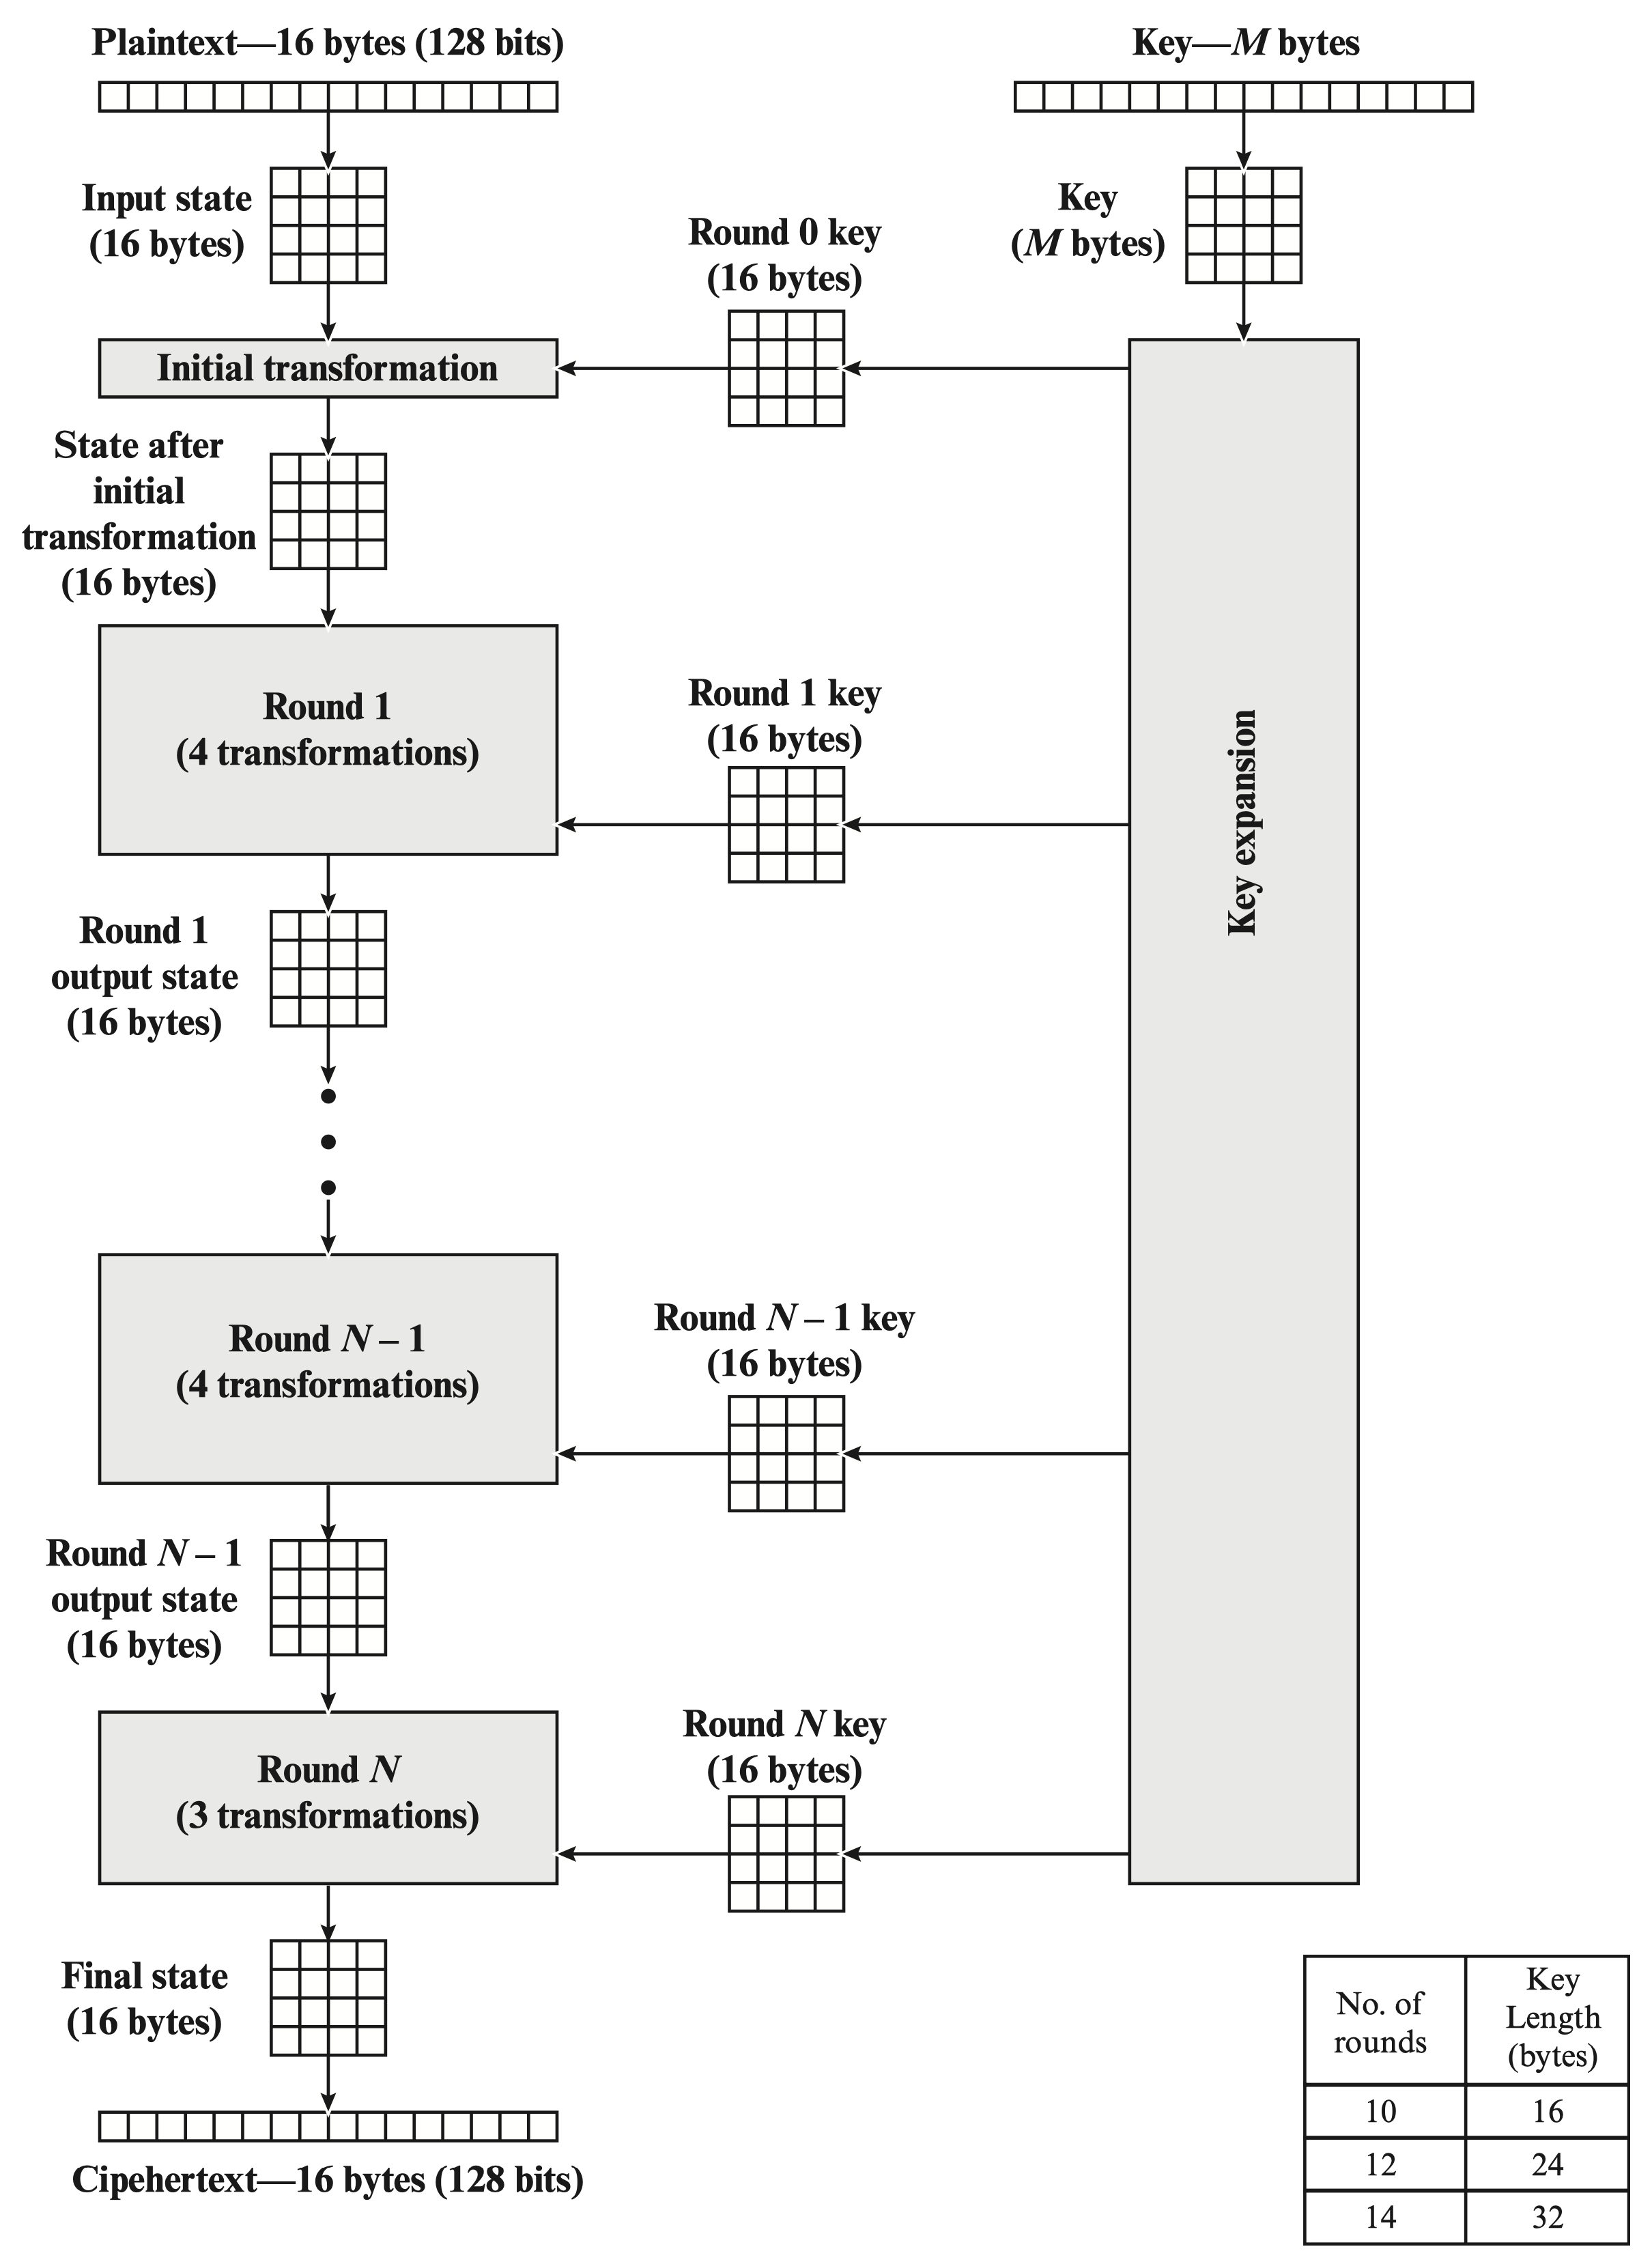
\includegraphics[width=0.66\linewidth]{2_aes_structure.jpg}
  \vspace{-4mm}
  \caption{AES Encryption Process} \label{fig:aes-encryption-process}
\end{figure}

\vspace{-4mm}

\begin{figure}[H]
  \centering
  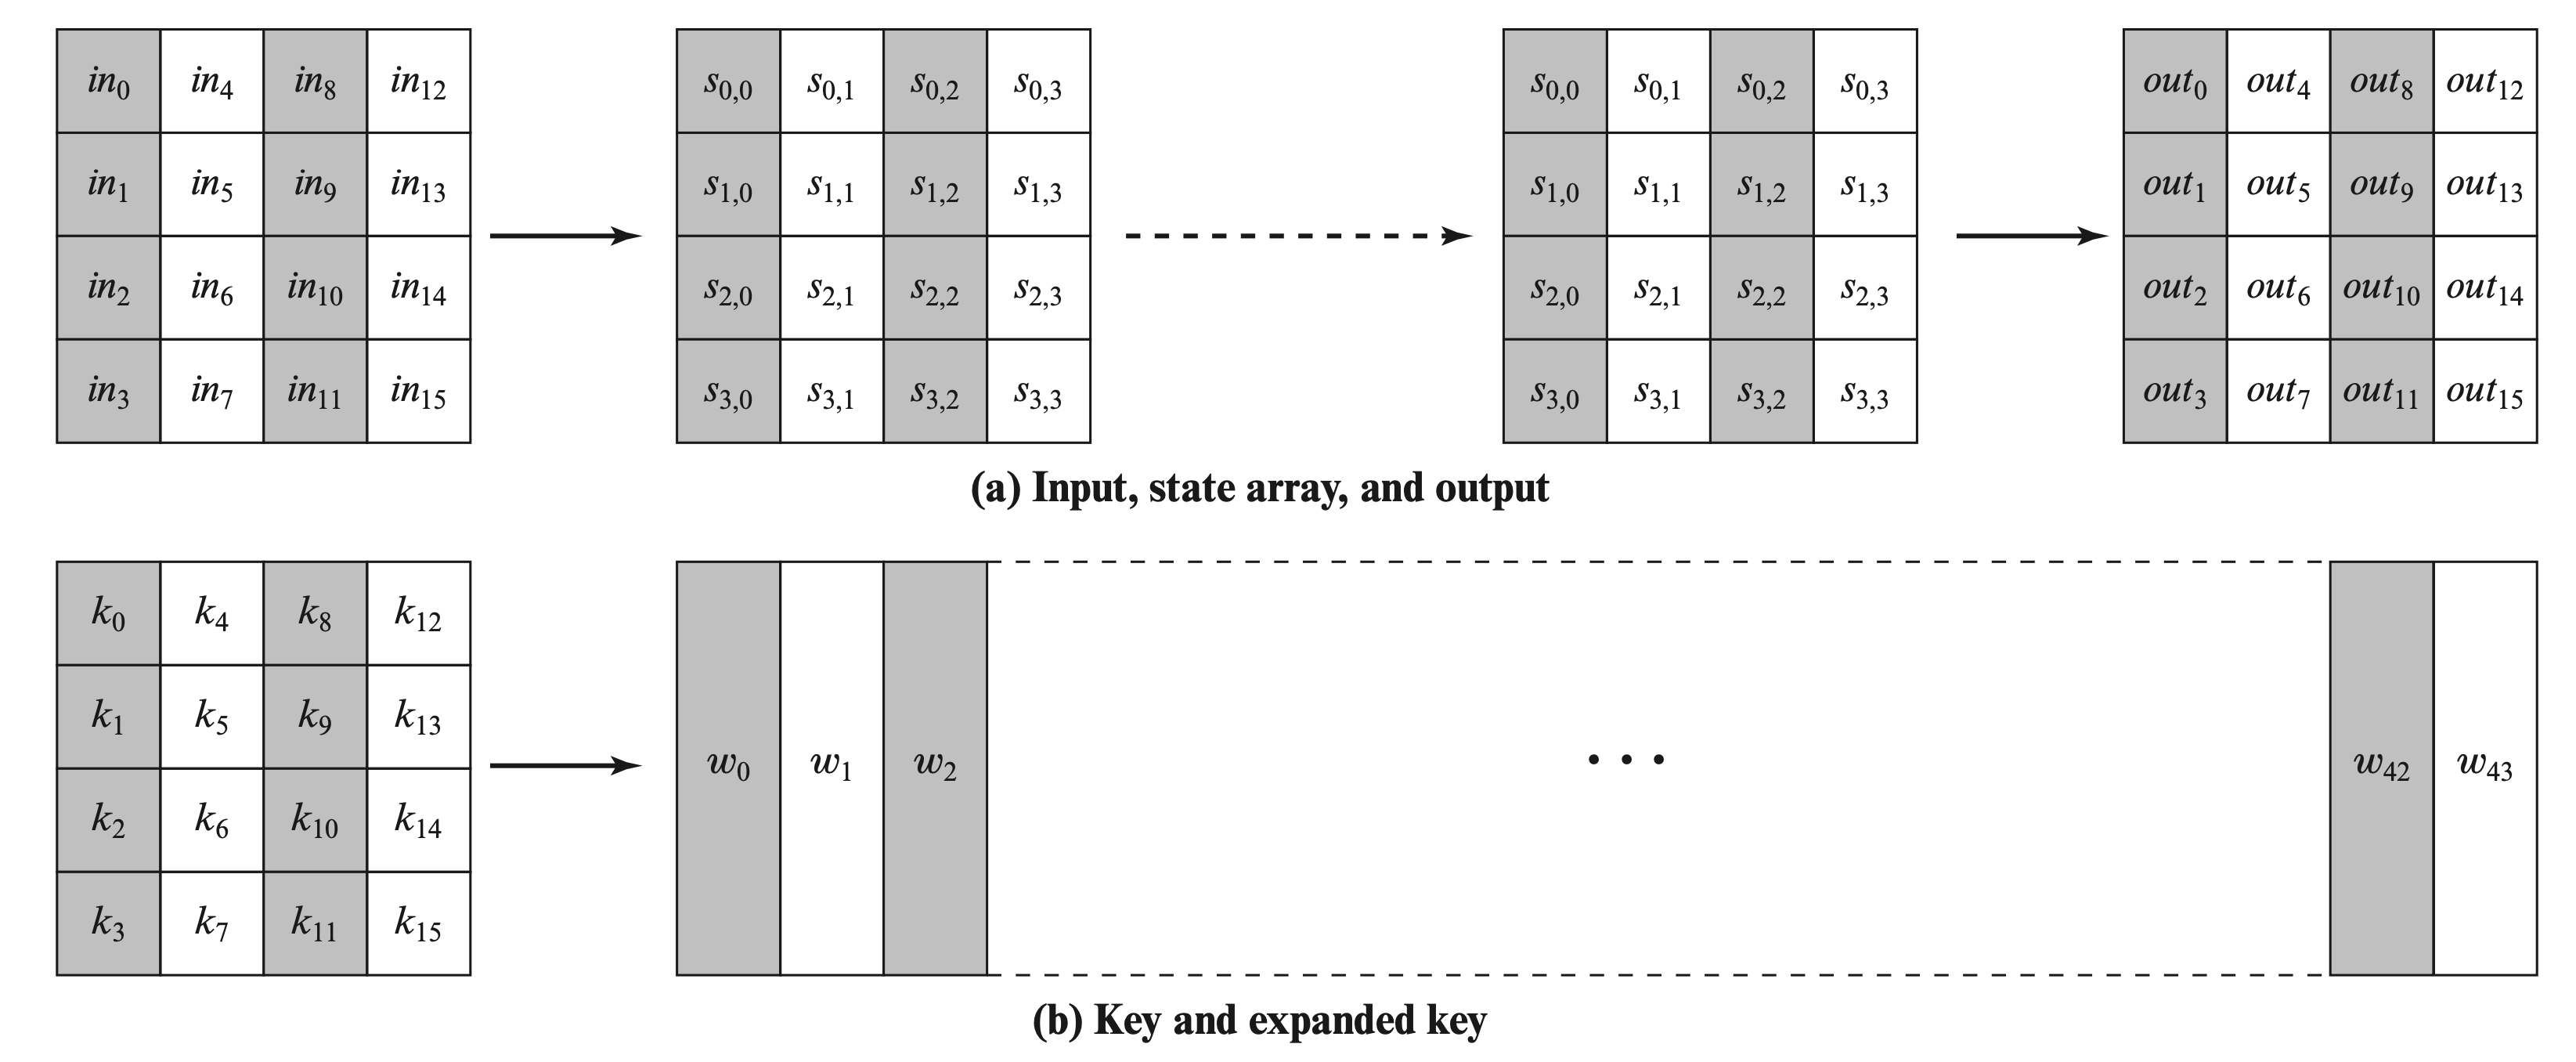
\includegraphics[width=0.975\linewidth]{2_aes_data_structure.jpg}
  \vspace{-3mm}
  \caption{AES Data Structure} \label{fig:aes-data-structure}
\end{figure}

\subsubsection{Struttura dettagliata}

La \figsubref{fig:aes-encryption-decryption}{a} mostra il cifrario AES più in dettaglio, indicando la sequenza di
trasformazioni in ciascun round e mostrando la corrispondente operazione di decryption.

\begin{figure}[H]
  \centering
  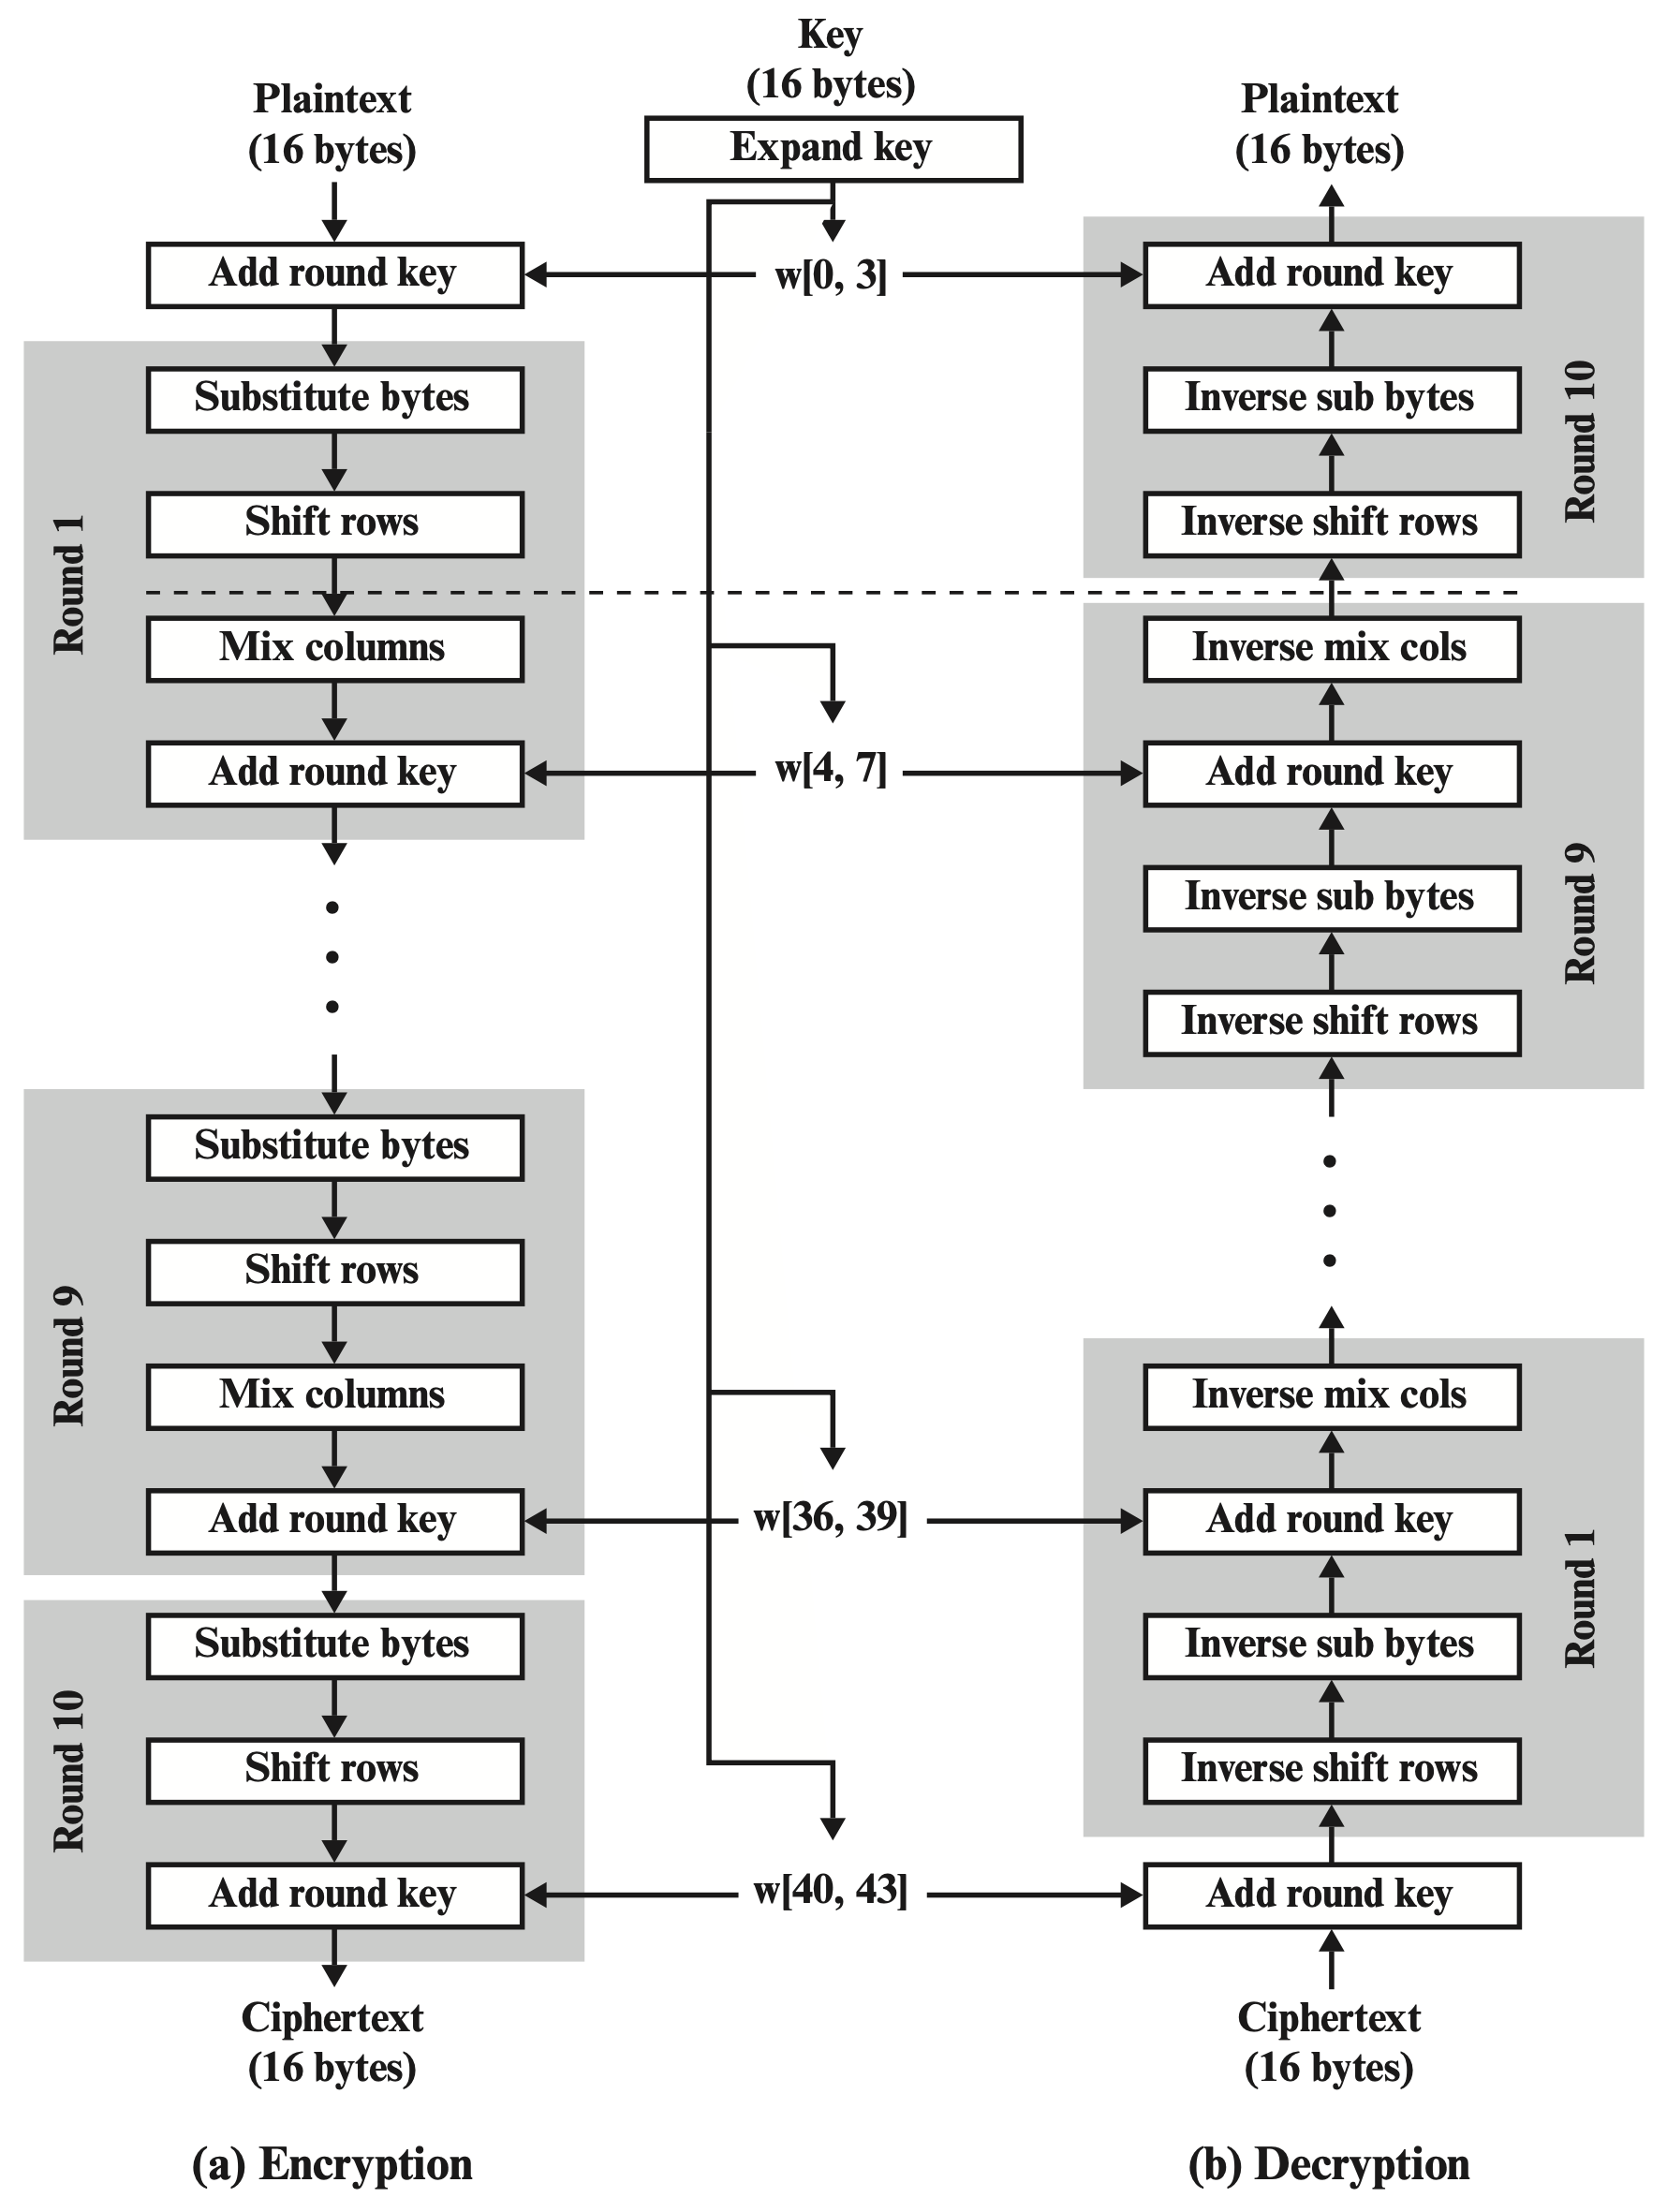
\includegraphics[width=0.7\linewidth]{2_aes_encryption_decryption.jpg}
  \vspace{-2mm}
  \caption{AES Encryption and Decryption} \label{fig:aes-encryption-decryption}
\end{figure}

Una prima osservazione importante è che AES non appartiene alla famiglia dei cifrari di Feistel. In una struttura di
Feistel, infatti, il blocco viene suddiviso in due metà, una delle quali viene usata per modificare l'altra, seguita
poi da uno scambio delle due parti. In AES, invece, l'intero blocco viene trattato in ogni round come un'unica matrice
di byte, sulla quale agiscono trasformazioni di sostituzione, permutazione e mescolamento lineare. Per questo motivo,
AES può essere ricondotto al paradigma delle \emph{Substitution-Permutation Networks} (SPN), pur presentando una
struttura specifica propria.

\begin{figure}[H]
  \centering
  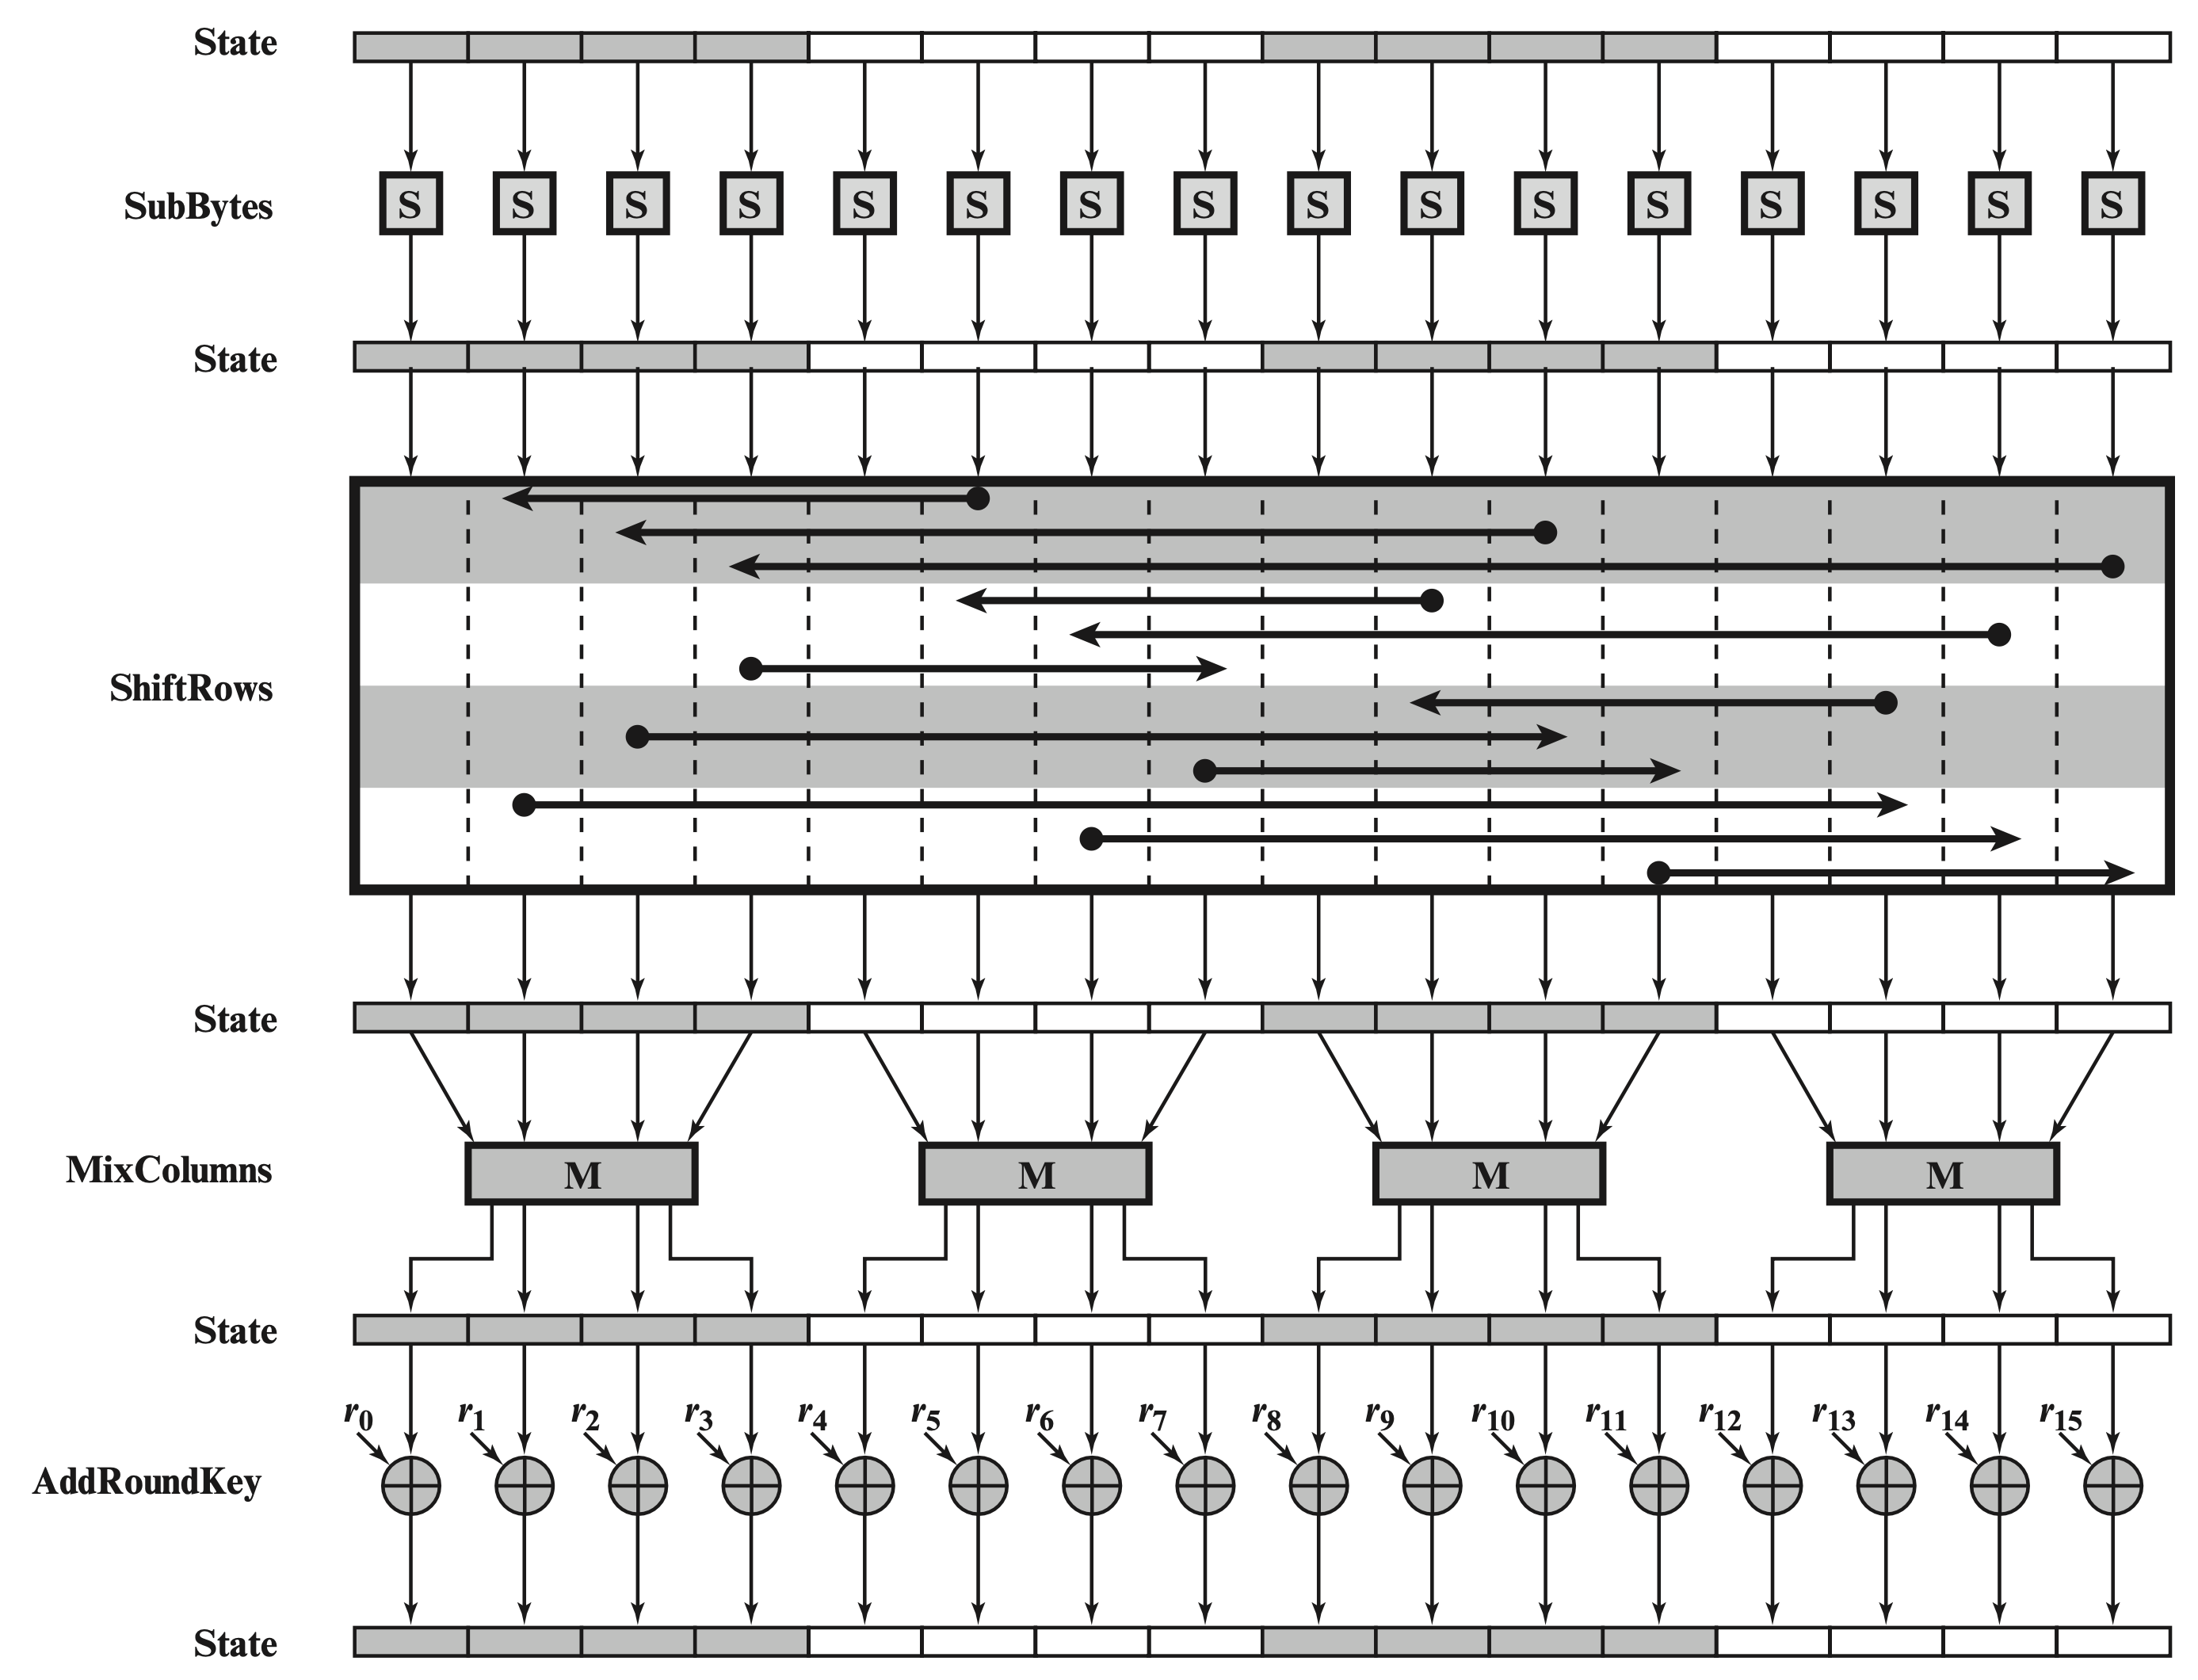
\includegraphics[width=0.85\linewidth]{2_aes_encryption_round.jpg}
  \vspace{-2mm}
  \caption{AES Encryption Round} \label{fig:aes-encryption-round}
\end{figure}

\subsection{Funzioni di trasformazione}

\subsubsection{Substitute Bytes}

\subsubsection{Shift Rows}

\subsubsection{Mix Columns}

\subsubsection{Add Round Key}

\subsection{Key Expansion}

\newpage
\part{Matematica}


\newpage
\input{chapters/03-matematica}

\end{document}



